
\documentclass{ximera}

%% Overschrijf theoremstyle (enkel in PDF, en enkel mogelijk in preamble!)
% \declaretheoremstyle[
%     headfont={\bfseries\sffamily\footnotesize},
%     notefont={\normalfont},
%     bodyfont={\normalfont},
%     headpunct={\relax},%\newline,
%     headformat={%
%         \makebox[0pt][r]{}{\bfseries \NAME\ \NUMBER \NOTE}},
% ]{definition}



\begin{document}
\title{Test layout en in/uitklappen}
\begin{abstract}
\end{abstract}
\maketitle

% \xmNewTheoremEnv{definition}
\xmNewTheoremEnv[box]{BoxI}
\XmTheoremDefaults{box}{expandable=true,nonumbered}
% \XmTheoremDefaults{box}{expandable=true,nonumbered, noprint}

\begin{tikzpicture}
  \draw[teal!70!black, postaction={decorate},
    decoration={markings, mark=at position 0.5 with {\gecentreerdepijl[3mm]}}]
    (0,0) -- (3,0);
\end{tikzpicture}

% \def\xmDebug{true}
\begin{tikzpicture}
   \poslading[Q_1]{q1}{0,0}
   \neglading[Q_2]{q2}{3,1.5}
   \drawvector[positie]{q1}{q2}{2}{$r_{12}$}
   \drawvector[snelheid]{q1}{30:1}{1.2}{$\vec{v}$}
   \drawvector[snelheidcomponent]{q1}{90:1}{1}{$\vec{v}_x$}
   \drawvector[kracht]{q1}{0:1}{1.2}{$\vec{F}$}
   \drawvector[krachtcomponent]{q1}{10:1}{1.2}{$\vec{F}_x$}
   \drawvector[versnelling]{q1}{-10:1}{1.2}{$\vec{a}$}
   \drawvector[versnellingcomponent]{q1}{-20:1}{1.2}{$\vec{a}_x$}
   \drawvector[Evector]{q1}{-30:1}{1.2}{$\vec{E}$}
   \drawvector[Evectorcomponent]{q1}{-40:1}{1.2}{$\vec{E}_x$}
   \drawvector[Eveldlijn]{q1}{-50:1}{2}{$E$}
   \drawvector[Mvector]{q1}{-60:1}{1.2}{$\vec{M}$}
   \drawvector[Mvectorcomponent]{q1}{-70:1}{1.2}{$\vec{M}_x$}
   \drawvector[Eveldlijn]{q1}{-80:1}{2}{$M$}
\end{tikzpicture}

            \begin{tikzpicture}
                \coordinate (O) at (0,0);
                \coordinate (Ftop) at (0,-3);

                % Assen onder 30° (evenwijdig/loodrecht met het hellend vlak)
                    \tekenassen[2.5]{O}{60}

                % De volledige zwaartekracht
                    \drawvector[kracht]{O}{Ftop}{3}{$\vec{F}_z$}

                % Ontbinden volgens de assen van het hellend vlak (hoek van de x-as: -60°)
                    \ontbindvector[krachtcomponent]{O}{Ftop}{-60}{$F_{z,x}$}{$F_{z,y}$}
            \end{tikzpicture}

% \begin{tikzpicture}
%    \node[charge] (Q1) at (0,0) {+};
%    %\node[charge+] (Q2) at (2,0) {charge+};
%    %\node[charge-] (Q3) at (4,0) {charge-};
%    \node(Q4) at (0,-2);
%    \poslading(Q4);
%    \draw[vector] (Q1) -- ++(0.8,0) node[above, midway]{$\vec{F}$};
%    \draw[vectorcomponent] (Q1) -- ++(0,-0.8) node[left, midway]{$\vec{F_x}$};
% \end{tikzpicture}
\section{Keuze van de chef}
\subsection{theorie}
\begin{definition}[foldable=true,title={Titel van definitie}]\nl
Definitie met titel, kan ingevouwen worden
\end{definition}
\begin{definition}[expandable=true,title={Titel van definitie}]\nl
Definitie met titel, kan uitgevouwen worden
\end{definition}

\begin{definition}
Definitie zonder titel
\end{definition}

\begin{proposition}[foldable=true,title={Titel van eigenschap}]\nl
eigenschap/theorie met titel, kan ingevouwen worden
\end{proposition}

\begin{proposition}
eigenschap/theorie zonder titel
\end{proposition}

\begin{remark}[foldable=true,title={Titel van opmerking}]\nl
opmerking met titel, kan ingevouwen worden
\end{remark}

\begin{remark}[expandable=true,title={Titel van opmerking}]\nl
opmerking met titel, kan uitgevouwen worden
\end{remark}

\begin{remark}
opmerking zonder titel
\end{remark}

%---------------
% QUIZ x: titel
\begin{question}
	Vraag met a, b, c, ...
	\begin{selectAll}
		\choice{$a$}
		\choice[correct]{$b$}
		\choice{$c$}
		\choice{$d$}
	\end{selectAll}

	\begin{solution}
		Uitleg
	\end{solution}
\end{question}
%---------------

\subsection{oefeningen}
%testen: \answer[onlineshowanswerbutton]{4}
\begin{exercise}\nl
Een enkelvoudige oefening
\begin{solution}
   antwoord met solution
\end{solution}
\end{exercise}

\begin{exercise}\nl
Een meervoudige oefening
\begin{question}
   Deel vraag 1
   \begin{solution}
      antwoord op deelvraag 1 met solution
   \end{solution}
\end{question}
\begin{question}
   Deel vraag 2
   \begin{hint}
      een hint
   \end{hint}
   \begin{solution}
      antwoord op deelvraag 2 met solution
   \end{solution}
\end{question}
\end{exercise}



\section{testjes}
\subsection{anders dan defenition}
\begin{proposition}[foldable=true,title={Behoud van ladingen}]\nl
Body   foldable (ie, expandable and expanded)
\end{proposition}

\begin{exercise}
Een oefening
\begin{solution}
   antwoord met solution
\end{solution}
\end{exercise}


\begin{question}
vraagstuk aze aze aze aze aze aze azle nazle nazken azlke zake azle azkle azkle jazklje lazj elkazje lkazj elkaz jelkazj e lkazj elkaz jelka zjelaz 
\end{question}


\begin{question}\nl
vraagstuk
\end{question}

\begin{question}\nl
Vraagstuk
\begin{solution}\nl
test met niets bij
\end{solution}
\end{question}

\subsection{expandeble en titels}
\subsubsection{zonder nl}
\begin{definition}[expandable=true,expanded,title={Veelterm, expandable and expanded}]
 Body expandable AND expanded (initially!)
\end{definition}

\begin{definition}[foldable=true,title={Veelterm, foldable (synonym for expandable and expanded)}]
 Body foldable (ie, expandable and expanded)
\end{definition}
\subsubsection{met nl}
\begin{definition}[expandable=true,expanded,title={Veelterm, expandable and expanded}]\nl
Body  expandable AND expanded (initially!)
\end{definition}

\begin{definition}[foldable=true,title={Veelterm, foldable (synonym for expandable and expanded)}]\nl
Body   foldable (ie, expandable and expanded)
\end{definition}

\section{vb van wim}
\begin{BoxI}[Veelterm,print=false]
  Body, print=false
\end{BoxI}
\begin{BoxI}[Veelterm]
Body  \verb|x^2|
\begin{itemize}
\item borderline
\end{itemize}
\end{BoxI}


\begin{BoxI}[title={Veelterm, not numbered},nonumbered]
Body no numbers
\end{BoxI}

\begin{BoxI}[title={Veelterm, not numbered not printed},noprint,nonumbered]
Body, no number, no print
\end{BoxI}

\begin{BoxI}
Body, no args
\end{BoxI}


\begin{definition}
Body no args
\end{definition}

\begin{proposition}
Body no args
\end{proposition}


\begin{definition}[Veelterm]
Body title Veelterm

Met een tweede lijn.
\end{definition}

\begin{definition}[title={Veelterm, met een lege lijn (en een komma en haakjes in de title)}]

 Body title Veelterm, met initiële lege lijn.

 En een tweede lijn.
\end{definition}

\begin{definition}[title={Veelterm, met een lege lijn EN nl (en een komma en haakjes in de title)}]\nl

 Body title Veelterm, met initiële lege lijn en de adhoc nl macro .

 En een tweede lijn.
\end{definition}

\begin{definition}[title={Veelterm, zonder een lege lijn maar MET nl (en een komma en haakjes in de title)}]\nl
 Body title Veelterm, met initiële lege lijn en de adhoc nl macro .

 En een tweede lijn.
\end{definition}


\begin{definition}[print=false,expandable=true,title={Veelterm, expandable and no print}]
Body noprint, expandable 
\end{definition}

\begin{definition}[expandable=true,expanded,title={Veelterm, expandable and expanded}]
Body noprint, expandable AND expanded (initially!)
\end{definition}

\begin{definition}[foldable=true,title={Veelterm, foldable (synonym for expandable and expanded)}]
Body noprint,  foldable (ie, expandable and expanded)
\end{definition}

\begin{definition}[print=false,expandable]
Body noprint, expandable, NO title
\end{definition}

\begin{definition}[print=false]
Body noprint,  NO title
\end{definition}

\begin{definition}[print=false,title={}]
Body noprint,  empty title
\end{definition}

\begin{definition}[expandable=true],title={Dit is een titel, met komma}]\nl
Body expandable=true, NO title; check the correct number after lot's of non-printing definitions!
\end{definition}

\begin{definition}[expandable],title={Dit is een titel, met komma}]\nl
Body expandable, NO title; Hopefully the title is not 'expandable' !!!
\end{definition}
\begin{definition}[expandable=true],title={Dit is een titel, met komma}]
Body expandable=true, NO title; check the correct number after lot's of non-printing definitions!
\end{definition}

\begin{definition}[expandable],title={Dit is een titel, met komma}]
Body expandable, NO title; Hopefully the title is not 'expandable' !!!
\end{definition}

\begin{definition}[{Titel, met komma's, en, haakjes maar zonder title is gelijk aan}]
Body, maar is de titel is waarschijnlijk FOUT. 
\end{definition}

\begin{definition}[Titel1, title={titel met toekenning aan 'titl'}, noexpandable, onbekendeoptiewordttitel]
Body met test titles
\end{definition}

\begin{definition}[Titel1, title={titel met toekenning aan 'title'}, noexpandable]
Body met test titles
\end{definition}


\begin{definition}[Met een explanation, hint en oplossing]
Body, met uitleg, hint en oplossing.
\begin{explanation} De uitleg (explanation) \end{explanation}
\begin{hint}        Een hint \end{hint}
% \begin{uitkomst}    De  uitkomst\end{uitkomst}
% \begin{oplossing}   De oplossing \end{oplossing}
\end{definition}

\begin{definition}[{Titel, met komma's, en, haakjes maar zonder title=}]
  Body, maar is de titel is waarschijnlijk FOUT. 
\end{definition}


Set definition by default expandable:
\XmTheoremDefaults{definition}{expandable=true}

\begin{definition}[Veelterm]
   no args, should expand because that is the default
\end{definition}

\begin{definition}[title={Veelterm, with noexpandable option}, noexpandable]
   This should NOT expand because the default is overwritten with noexpandable
\end{definition}

Set Options
    \tcbset{default-style/.style={
              boxrule     = 5pt,
              boxsep      = 5pt,
              rounded corners,
      } 
    }
    
\colorlet{theory}{red}

\begin{definition}[Veelterm]
   Een veelterm ...
\end{definition}

\begin{definition}[Veelterm]
   Een veelterm ...
\end{definition}

\begin{theorem}[Veelterm]
   Een veelterm ...
\end{theorem}




\begin{example}[Een derdegraadsveelterm met vier nulpunten ]

    Dat bestaat niet echt ...
\end{example}

\begin{remark}[Een derdegraadsveelterm met vier nulpunten ]

    Dat bestaat echt niet ...
\end{remark}

\begin{remark}[expandable]

    Een uitklapbare opmerking zonder 'titel'.
\end{remark}

\end{document}

